\documentclass[11pt]{article}
\usepackage[margin=1in]{geometry}
\usepackage{amsmath,amssymb}
\usepackage{booktabs}
\usepackage{graphicx}
\usepackage{xcolor}
\usepackage{caption}
\setlength{\parindent}{0pt}\setlength{\parskip}{6pt}

\begin{document}
{\large\bfseries Critic agent and its validation --- copy-paste text for the paper}\\
{\small Only the critic part. Paste the marked blocks into \emph{Materials and
Methods} and \emph{Result and Discussion}. Replace numbers later if re-run.}

\hrulefill

\textcolor{blue}{\bfseries [PASTE INTO: Materials and Methods]}

\textbf{Critic agent.} The critic first solves each item independently, then
scores it on five dimensions---correctness, distractor quality, difficulty
alignment, language quality, and technical validity (\LaTeX{} rendering for
mathematics; figure relevance for image items)---each in $[0,10]$.
The overall score is the weighted mean
\begin{equation}
S=\frac{\sum_{d} w_d s_d}{\sum_{d} w_d},\qquad w_{\text{correctness}}=3,\ w_{\text{others}}\in\{1,2\},
\end{equation}
and an item is accepted when $S\ge\theta$ ($\theta=6$).

\textbf{Multi-critic ensemble.} To reduce single-model self-evaluation bias we
aggregate $K=3$ heterogeneous critics (Gemini-3.1-Pro, GPT-5.5,
Claude-Sonnet-4.6): the answer is the majority vote, each dimension the mean
over critics, and inter-critic reliability is reported with Cohen's $\kappa$,
\begin{equation}
\kappa=\frac{p_o-p_e}{1-p_e}.
\end{equation}
For mathematics a sandboxed SymPy verifier checks the answer \emph{before} the
LLM critic; figure-dependent items are routed to a vision-capable critic.

\textbf{Expert-free validation (Critic Discrimination Index).} We validate the
critic \emph{without} human grading by injecting known faults. From each real
national-test item we synthesise two degraded variants---\textsc{wrong-key}
(key relabelled to a distractor) and \textsc{weak-distractors} (two distractors
replaced by implausible fillers)---and measure the paired score drop on
dimension $d$,
\begin{equation}
\mathrm{CDI}_d=\frac1N\sum_{i=1}^{N}s_d^{\text{real}}(i)-\frac1N\sum_{i=1}^{N}s_d^{\text{deg}}(i).
\end{equation}
A valid critic gives a large positive $\mathrm{CDI}$ on the targeted dimension
and $\approx 0$ elsewhere. Significance uses the two-sided Wilcoxon signed-rank
test and effect size the paired Cohen's $d=\overline{\Delta}/s_\Delta$ with
$\Delta_i=s_d^{\text{real}}(i)-s_d^{\text{deg}}(i)$.

\hrulefill

\textcolor{blue}{\bfseries [PASTE INTO: Result and Discussion]}

Across both subjects and all three critics the discrimination is statistically
significant with large effect sizes: relabelling the key collapses the
correctness score and weakening the distractors collapses the
distractor-quality score, exactly as a valid critic should behave
(Tables~\ref{t1}--\ref{t2}, Fig.~\ref{f1}). On figure-dependent mathematics
items the critic answered $6/9$ correctly without the image but $9/9$ with the
vision critic (Table~\ref{t3}).

\begin{table}[h]\centering\caption{CDI --- mathematics ($N\!\approx\!40$/model; all $p<0.001$).}\label{t1}
\begin{tabular}{lccc}
\toprule
Critic & Solve acc. & wrong-key $\to$ correctness (gap, $d$) & weak-distr. $\to$ distractor q. (gap, $d$)\\
\midrule
Claude-Sonnet-4.6 & 0.98 & $+8.85\ (4.94)$ & $+3.03\ (1.53)$\\
Gemini-3.1-Pro & 0.95 & $+8.58\ (2.95)$ & $+5.10\ (1.50)$\\
GPT-5.5 & 1.00 & $+8.73\ (2.75)$ & $+2.99\ (1.69)$\\
\bottomrule
\end{tabular}\end{table}

\begin{table}[h]\centering\caption{CDI --- Kazakh language ($N\!=\!20$/model; all $p\le0.0002$).}\label{t2}
\begin{tabular}{lccc}
\toprule
Critic & Solve acc. & wrong-key $\to$ correctness (gap, $d$) & weak-distr. $\to$ distractor q. (gap, $d$)\\
\midrule
Claude-Sonnet-4.6 & 0.75 & $+5.15\ (1.73)$ & $+4.60\ (3.87)$\\
Gemini-3.1-Pro & 0.90 & $+8.15\ (1.87)$ & $+7.90\ (4.07)$\\
GPT-5.5 & 0.80 & $+6.70\ (1.69)$ & $+3.90\ (2.99)$\\
\bottomrule
\end{tabular}\end{table}

\begin{table}[h]\centering\caption{Vision ablation (figure-dependent math items).}\label{t3}
\begin{tabular}{lcc}
\toprule
Critic & Blind (no image) & With image\\
\midrule
Claude-Sonnet-4.6 & $2/3$ & $3/3$\\
Gemini-3.1-Pro & $1/3$ & $3/3$\\
GPT-5.5 & $3/3$ & $3/3$\\
\textbf{Total} & $\mathbf{6/9}$ & $\mathbf{9/9}$\\
\bottomrule
\end{tabular}\end{table}

\begin{figure}[h]\centering
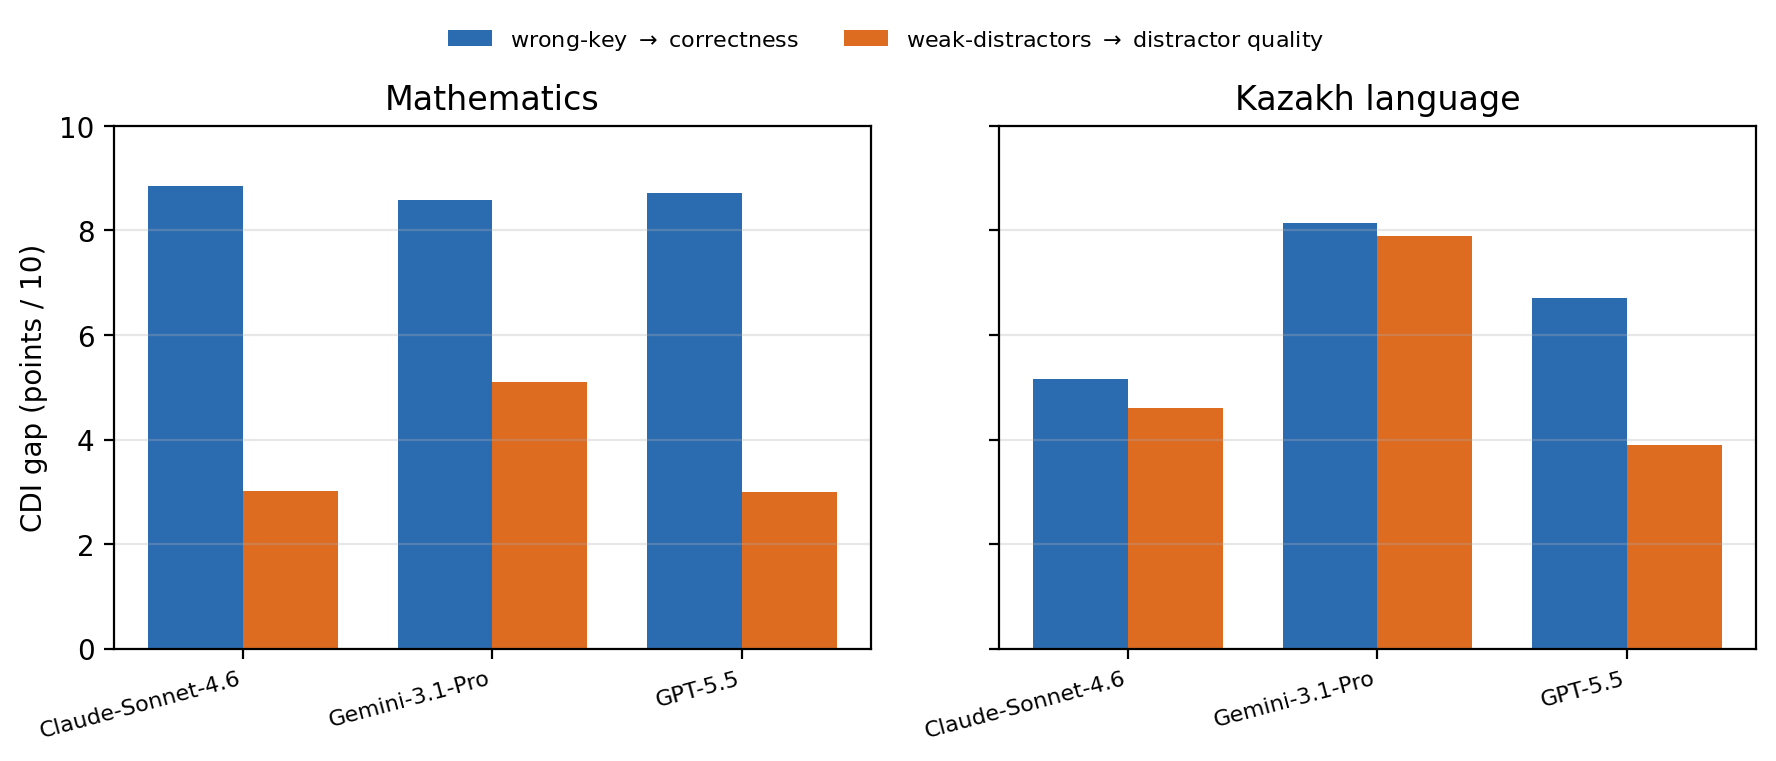
\includegraphics[width=0.92\linewidth]{fig_cdi.png}
\caption{CDI (gap between real and degraded mean scores) by model and subject.}\label{f1}
\end{figure}

\textbf{Limitations to note:} CDI is a proxy for human judgement
(expert-correlation is future work); the vision ablation is small ($n=3$
image items per model).

\end{document}
